\chapter{Spatial Decomposition}{\label{ch:Spatial Decomposition}
  \def\figpath{chapters/05/figures/}
  \graphicspath{ {\figpath} }
  %%%%%%%%%%%%%%%%%%%%%%%%%%%%%%%%%%%%%%%%%%%%%%%%%%%%%%%%%%%%%%%%%%%%%%%%%%%%%%
  % Introduction
  %%%%%%%%%%%%%%%%%%%%%%%%%%%%%%%%%%%%%%%%%%%%%%%%%%%%%%%%%%%%%%%%%%%%%%%%%%%%%%
  \section{Introduction}{\label{sec:Spatial Decomposition:Introduction}
    Until relatively recently, the method of choice for neutronics calculations has been neutron diffusion.
    Neutron diffusion codes can perform whole-core calculations, on a typical workstation, in relatively short run-times.
    However, with the recent shift towards higher fidelity methods such as \ac{SN}, and \ac{MOC} \cite{Askew1972}, more significant computational resources are necessary.
    These high fidelity methods allow for more detailed analysis, through finer resolution and use of fewer approximations, but typically take far more time to perform calculations; particularly for large calculations.
    Although processor clock-speeds have significantly improved, in the past several years processors have, for the most part, not gotten faster.
    To reduce the run-times (real-time) of high fidelity simulations, it is thus necessary to rely on parallelism.

    There are many different aspects of parallelism, and thread-based parallelism has been discussed previously \cref{sec:MOC:Parallelism}.
    This type of parallelism (thread), is limited to the resources of a single computational node.
    In order to utilize more resources, it is necessary to use a technique called \emph{domain decomposition}.
    Even without considerations for run-times, these high-fidelity simulations typically use more memory than is available on a single node, and domain decomposition becomes a necessity.
    In general, domain decomposition involves splitting up one domain of the problem into smaller subdomains; some typical domains to decompose are space, direction, and energy.
    Each smaller subdomain is assigned to a separate processor, and these can be run in parallel; although, there is generally some communication between the processors.

    In Monte-Carlo simulations, it is common that spatial decomposition involves duplication of some spatial locations [CITATION].
    However, in deterministic transport methods, each domain is typically \emph{partitioned}, that is the domain is split without any overlap between subdomains.
    The MPACT \cite{MPACT2016} code has the ability to decompose two domains: space and direction.
    In MPACT, each discrete direction has a calculable amount of work, and the decomposition is trivial; in general, the same cannot be said of the spatial domain.
    This chapter focuses on improvements to the spatial decomposition techniques used in MPACT; these techniques, however, can be applied to other transport codes and similar results would be expected.
    The contents of this chapter are, in large part, adapted from an article published on this work \cite{Fitzgerald2019a}.

    As diffusion has been the method of choice for so long in the reactor physics field, spatial partitioning techniques common in other fields have, largely, not been applied.
    Transport codes such as MPACT \cite{MPACT2016}, or OpenMOC \cite{Gunow2018} used simple spatial partitioning methods that divided the core into uniformly sized blocks.
    However, the spatial partitioning of a reactor can be abstracted to a graph partitioning problem \cite{Fitzgerald2017}, which has been well studied in computer science \cite{Elsner1997} and applied to other simulation fields such as computational fluid dynamics \cite{Yao1998}.
    In general, the graph partitioning problem is NP-complete, meaning that a partitioning cannot be easily verified as optimal; therefore, graph partitioning relies on approximate heuristic methods.
    Many different methods have been developed for graph partitioning, several of which are discussed in \cref{sec:Spatial Decomposition:Applied Graph Theory}.

    The remained of this chapter is structured as follows.
    In \cref{sec:Spatial Decomposition:Spatial Decomposition in MPACT}, a description of spatial decomposition in MPACT is given.
    \Cref{sec:Spatial Decomposition:Applied Graph Theory} introduces relevant graph theory concepts, and the methods used for spatial partitioning in this work.
    \Cref{sec:Spatial Decomposition:Applications for MPACT} describes the applications of these graph theory methods in MPACT.
    \Cref{sec:Spatial Decomposition:Results} compares methods for 2-D and 3-D reactor simulations.
    Finally, \cref{sec:Spatial Decomposition:Conclusions} lists the conclusions that are drawn from this work.
  }
  %%%%%%%%%%%%%%%%%%%%%%%%%%%%%%%%%%%%%%%%%%%%%%%%%%%%%%%%%%%%%%%%%%%%%%%%%%%%%%
  % Spatial Decomposition in MPACT
  %%%%%%%%%%%%%%%%%%%%%%%%%%%%%%%%%%%%%%%%%%%%%%%%%%%%%%%%%%%%%%%%%%%%%%%%%%%%%%
  \section{Spatial Decomposition in MPACT}{\label{sec:Spatial Decomposition:Spatial Decomposition in MPACT}
    MPACT is a neutron transport code, based on the \ac{MOC}.
    It was originally developed for direct whole-core simulation of \acp{LWR}.
    In the \ac{MOC}, an approximate transport equation is solved analytically along characteristic rays that traverse the problem.
    By using many of these characteristic rays, an accurate solution is obtained; however, storing the data of these characteristic rays can use a considerable amount of memory.

    In MPACT, the modular ray-tracing technique \cite{Saji2000} is used to reduce the memory used for storing characteristic ray information.
    Modular ray-tracing involves dividing the reactor system into \emph{ray-tracing modules}, which are small geometries that are often repeated in the reactor.
    Characteristic rays are constructed in each ray-tracing module such that each ray directly links to a ray in an adjacent module.
    In this method, characteristic ray information is only stored for each \emph{unique} ray-tracing module.

    Ray-tracing modules are the smallest unit for spatial decomposition in MPACT \cite{StimpsonPartitioning2017}.
    These ray-tracing modules are typically an axial slice of a quarter of a full fuel assembly, as shown in \cref{fig:Spatial Decomposition:5a-2d abstraction}
    The core consists of a structured grid of these modules in which each module has the same dimensions but may have different numbers of computational cells.
    Therefore, in MPACT, the spatial decomposition is a structured grid partitioning problem.

    In general, it is possible to use the computational cells as the smallest unit in the decomposition.
    However, this causes the decomposition problem to become an unstructured mesh partitioning problem.
    This is not done in MPACT because communication would become significantly more complicated.
    Additionally, there would be more re-entrant rays which would have negative impacts on the rate of convergence.

    \begin{figure}
      \centering
      \begin{subfigure}[t]{0.45\textwidth}
        \centering
        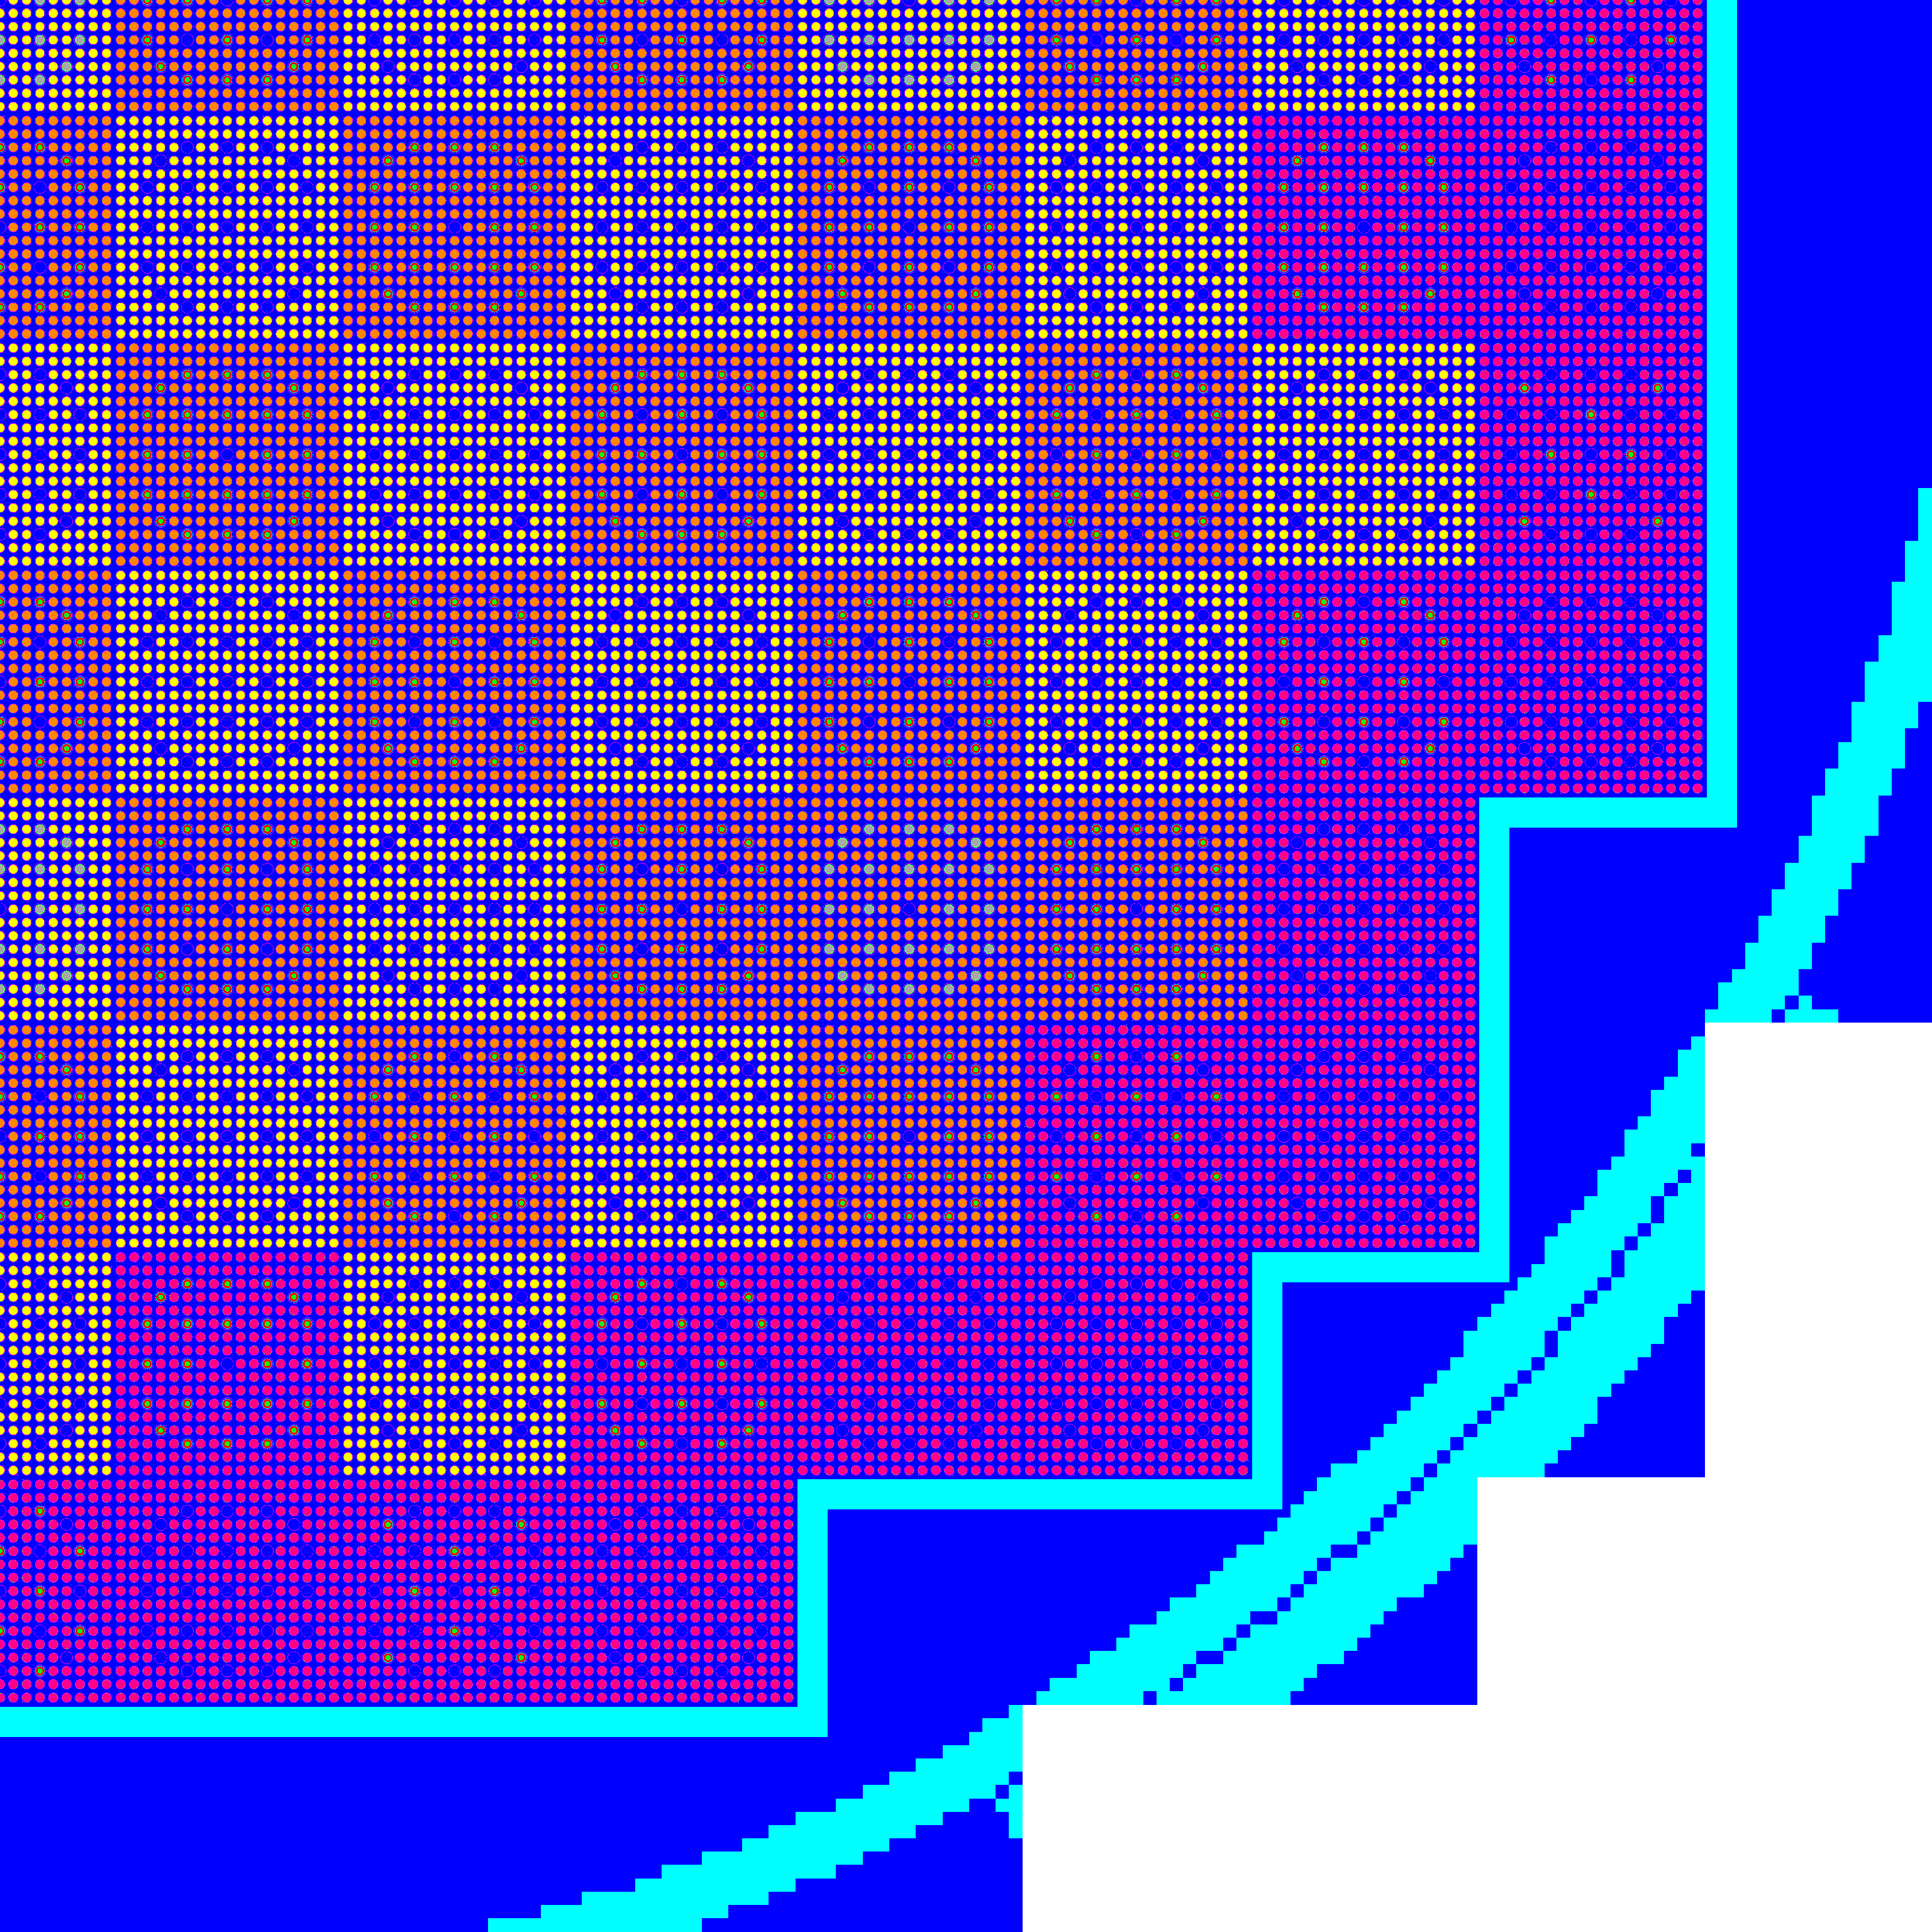
\includegraphics[width=0.9\textwidth]{5a-2d_core}
        \caption{fine mesh\label{fig:Spatial Decomposition:5a-2d configuration}}
      \end{subfigure}%
      ~
      \begin{subfigure}[t]{0.45\textwidth}
        \centering
        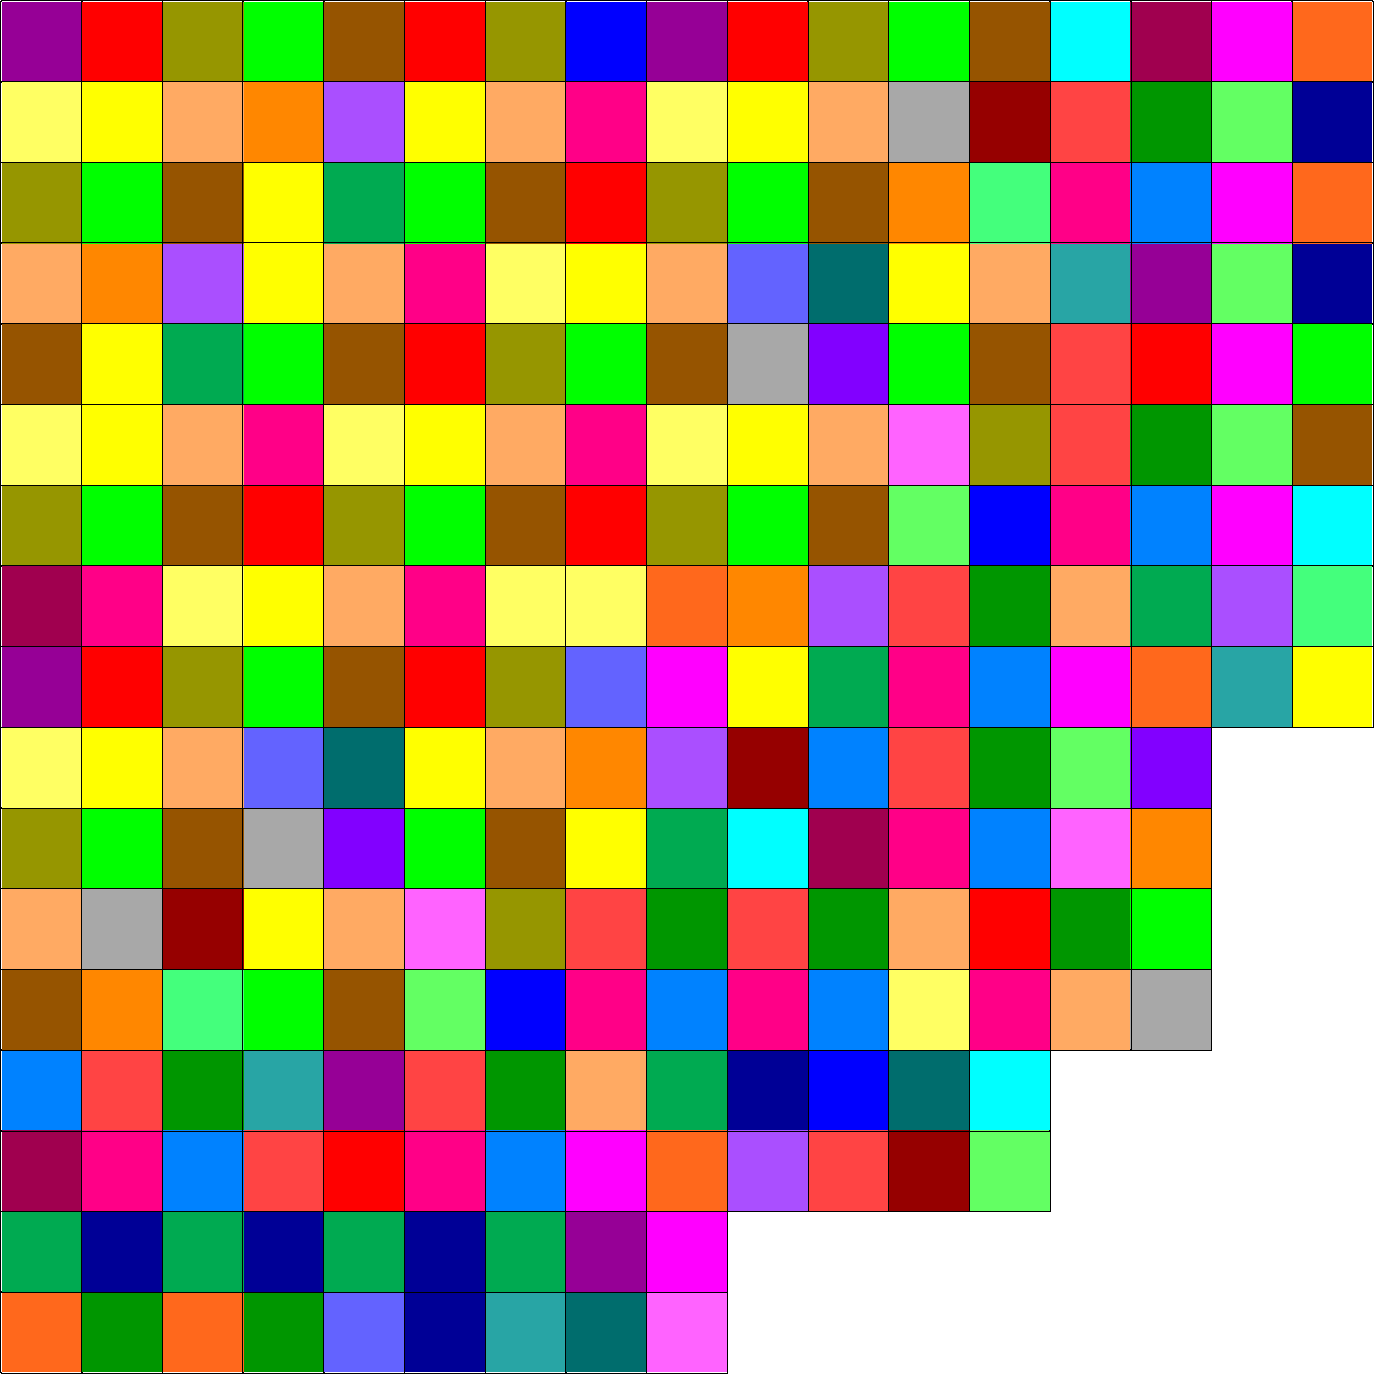
\includegraphics[width=0.9\textwidth]{modmesh_5a-2d}
        \caption{ray-tracing module mesh\label{fig:Spatial Decomposition:5a-2d modular mesh}}
      \end{subfigure}
      \caption{Example quarter core configuration and corresponding ray-tracing modular mesh in MPACT. \label{fig:Spatial Decomposition:5a-2d abstraction}}
    \end{figure}

    MPACT has had two spatial decomposition methods in the past: manual decomposition, and assembly-based decomposition.
    A user may manually enter a decomposition \cite{StimpsonPartitioning2017}, but it is time consuming to construct a balanced decomposition and will likely still be suboptimal to some degree.
    An automated method exists that recursively bisects the core using Morton-ordering \cite{Morton1966} applied to the reactor assembly geometries.
    While this method is automated, it often yields very imbalanced domains, and also restricts the number of subdomains that can be used.

    Previous work has shown that spatial decomposition of reactors can be abstracted to a graph partitioning problem \cite{Fitzgerald2017}.
    The use of graph partitioning methods in MPACT is expected to solve the issues encountered in each of the two approaches described above.
    These methods can be used to decompose into an arbitrary number of domains with high quality results, without user input.

    Existing graph partitioning libraries such as METIS \cite{METIS} partition graphs very efficiently and have very high quality results.
    To use all given processors, MPACT requires that each spatial subdomain contains at least one module, i.e. no partition can be empty.
    However, in some cases, particularly when the number of partitions is high, METIS may generate empty partitions.
    This means METIS cannot be used to decompose the core into an arbitrary number of subdomains without modifying the resulting partitions.
    For this reason, MPACT does not rely on third-party libraries for graph partitioning in the spatial decomposition process.
  }
  %%%%%%%%%%%%%%%%%%%%%%%%%%%%%%%%%%%%%%%%%%%%%%%%%%%%%%%%%%%%%%%%%%%%%%%%%%%%%%
  % Applied Graph Theory
  %%%%%%%%%%%%%%%%%%%%%%%%%%%%%%%%%%%%%%%%%%%%%%%%%%%%%%%%%%%%%%%%%%%%%%%%%%%%%%
  \section{Applied Graph Theory}{\label{sec:Spatial Decomposition:Applied Graph Theory}
    The spatial decomposition of a reactor core can be abstracted to the partitioning of a graph.
    Specifically, this would be a weighted graph, $G(V,E)$, which is comprised of a set of vertices, $V$, and a set of edges, $E$, that connect pairs of vertices.
    In general, these vertices and edges may have weights; a vertex $v_i$ will have weight $w_i$, and an edge $e_i$ between vertices $v_i$ and $v_j$ will have weight $c_{ij}$.
    In MPACT, a vertex represents a ray-tracing module, and the edges represent communication between adjacent modules in the \ac{MOC}.
    The graphs are undirected because communication between ray-tracing modules is two-way.

    Previous work \cite{Fitzgerald2017} applied unweighted graph partitioning techniques to the reactor spatial decomposition problem; the work presented here applies generalizations and improvements to the methods used for graphs with weighted vertices and edges.
    A vertex's weight indicates the amount of computational work that is needed; as one might expect, this is highly correlated with the number of computational cells.
    This is shown in \cref{sec:Spatial Decomposition:Results}.
    In general, the edges may also be weighted to account for different amounts of data transfer.
    This is discussed in more detail in \cref{sec:Spatial Decomposition:Applications for MPACT}.

    The goal is for each partition to have equal weight, with minimal weight of edges cut by partition boundaries.
    This is equivalent to each subdomain having the same amount of computational work with minimized communication between processes.
    If each process has roughly the same amount of work to perform, then less time will be spent waiting for other processes, thus improving parallel efficiency.
    Also, with less communication, less time will be spent passing data between processes, so the parallel overhead will be reduced.

    In this work, methods were separated into two distinct categories: partitioning methods and partition refinement (improvement) methods.
    Partitioning methods give a near-balanced partitioning for a given graph.
    Refinement methods attempt to reduce communication between existing partitions in a graph.
    As applied in MPACT, these refinement methods typically did not significantly reduce communication.
    These methods and results are presented in \cref{sec:Spatial Decomposition:Partition Refinement}.
    %%%%%%%%%%%%%%%%%%%%%%%%%%%%%%%%%%%%%%%%%%%%%%%%%%%%%%%%%%%%%%%%%%%%%%%%%%%%
    % Graph Partitioning Methods
    %%%%%%%%%%%%%%%%%%%%%%%%%%%%%%%%%%%%%%%%%%%%%%%%%%%%%%%%%%%%%%%%%%%%%%%%%%%%
    \subsection{Graph Partitioning Methods}{\label{ssec:Spatial Decomposition:Graph Partitioning Methods}
      In this work, recursive partition methods were considered due to their capability to partition into arbitrary numbers of domains.
      Each of these recursive partitioning methods sorts the graph, using different methods, and then divides or ``cuts'' the graph into two subgraphs with approximately equal vertex weights.
      Once a graph's vertices are sorted into a list, $V_s$, the graph can be bisected using \cref{alg:Graph Cutting}.

      Multi-level partitioning methods are widely used in other fields such as networking, where graphs can become very large; however, in MPACT, the number of ray-tracing modules is on the order of a few hundred to several thousand, which directly correlates to the size of the graph.
      Additionally, for MPACT, the decomposition problem is static, so the computation time for partitioning is expected to be negligible as it can simply be performed one time at the outset.
      Due to the small graph size, multi-level methods were not considered as part of this work.

      \begin{algorithm}[ht]
        \centering
        \caption{The algorithm used to determine how to cut a graph, $G(V,E)$, into two subgraphs based on a sorted vertex list $V_s$, and that the graph will be recursively partitioned into $N$ groups.}
        \label{alg:Graph Cutting}
        \begin{algorithmic}[1]
          \Procedure{Graph Cut}{$G(V,E), V_s, N$}
            \State{$N_1 \gets \floor{N/2}$} \Comment{Desired number of recursive partitions for first subgraph}
            \State{$W_1 \gets \frac{N_1}{N}\suml[v_i\in V]w_i$} \Comment{Ideal weight of first subgraph}
            \State{Let $V_1$ be a set of vertices such that:
                \begin{itemize}[leftmargin=1.5cm]
                    \item{$V_1 \subset V$}
                    \item{The vertices $V_1$ are taken in order from $V_s$}
                    \item{$W_1 - \suml[v_i\in V_1] w_i$ is minimized}
                \end{itemize}
            }
            \State{Let $V_2$ be the subset $V \setminus V_1$}
            \State{Optionally call a refinement method}
            \State{Create a graph $G_1$ from $V_1$}
            \State{Create a graph $G_2$ from $V_2$}
          \EndProcedure
        \end{algorithmic}
      \end{algorithm}
      %%%%%%%%%%%%%%%%%%%%%%%%%%%%%%%%%%%%%%%%%%%%%%%%%%%%%%%%%%%%%%%%%%%%%%%%%%
      % Recursive Spectral Bisection
      %%%%%%%%%%%%%%%%%%%%%%%%%%%%%%%%%%%%%%%%%%%%%%%%%%%%%%%%%%%%%%%%%%%%%%%%%%
      \subsubsection{Recursive Spectral Bisection}{\label{sssec:Spatial Decomposition:Recursive Spectral Bisection}
        The \ac{RSB} method, originally developed by \citet{Pothen1989}, has been highly successful and widely used in graph partitioning \cite{Simon1991,Spielman2007}.
        This method relies entirely on the connectivity of the graph and not on its geometry.
        The \ac{RSB} method has been improved to allow to allow for partitioning of \emph{weighted} graphs into any number of domains \cite{Hsieh1995}.

        The \ac{RSB} method makes use of the Laplacian matrix of a graph; specifically the second-smallest eigenvalue of this matrix, referred to by Fiedler as the \emph{algebraic connectivity} \cite{Fiedler1973}.
        The eigenvector associated with this eigenvalue has also been known as the \emph{Fiedler vector}.
        For weighted graphs, the weighted Laplacian matrix is used in lieu of the Laplacian matrix; matrix elements are given by
        \begin{align}
          \label{eq:Spatial Decomposition:Weighted Laplacian}
          L_{ij} =
            \begin{cases}
              d_i, \quad&{i=j},\\
              c_{ij}, \quad&{i\neq j},\\
              0, \quad&{\text{else}},
            \end{cases}
        \end{align}
        where $d_i$ is the sum of edge weights from vertex $v_i$, and $c_{ij}$ is the weight of the edge between vertices $v_i$ and $v_j$.
        The Fiedler vector is found from this weighted Laplacian matrix; by sorting the values of the Fiedler vector, the vertices can be reordered in a one-dimensional list $V_s$.
        This list of vertices is then divided into two sets, based on weight and total number of partitions needed (see \cref{alg:Graph Cutting}).
        The recursive spectral bisection algorithm is listed in \cref{alg:Recursive Spectral Bisection}.

        \begin{algorithm}
          \centering
          \caption{The recursive spectral bisection (RSB) algorithm.}
          \label{alg:Recursive Spectral Bisection}
          \begin{algorithmic}[1]
            \Procedure{RSB}{$G(V,E)$}
              \State{Let $L$ be the weighted Laplacian of $G(V,E)$}
              \State{Compute eigenvectors of $L$}
              \State{Use the Fiedler vector to sort $V\to V_s$} \Comment{If tie, use larger eigenvectors}
              \State{Cut graph into $G_1(V_1,E_1), G_2(V_2,E_2)$: \Cref{alg:Graph Cutting}}
              \State{RSB($G_1(V_1,E_1)$)}
              \State{RSB($G_2(V_2,E_2)$)}
            \EndProcedure
          \end{algorithmic}
        \end{algorithm}
      }
      %%%%%%%%%%%%%%%%%%%%%%%%%%%%%%%%%%%%%%%%%%%%%%%%%%%%%%%%%%%%%%%%%%%%%%%%%%
      % Recursive Inertial Bisection
      %%%%%%%%%%%%%%%%%%%%%%%%%%%%%%%%%%%%%%%%%%%%%%%%%%%%%%%%%%%%%%%%%%%%%%%%%%
      \subsubsection{Recursive Inertial Bisection}{\label{sssec:Spatial Decomposition:Recursive Inertial Bisection}
        Another class of recursive partitioning methods are coordinate or geometric methods.
        There are many different geometric partitioning methods in existence; in this study, the \ac{RIB} method \cite{Elsner1997,Floros1995} was investigated.
        This method uses only the geometry of the graph to construct a bisector and does not consider the connectivity (edges) in any way.

        The \ac{RIB} method determines a bisector which cuts the graph into two approximately equally sized subdomains.
        This is easily generalized for weighted graphs.
        The bisector should have approximately equal amounts of weight on each side.
        The \ac{RIB} makes no assumption of the orientation of the graph in space, unlike some other coordinate partitioning methods.
        The principle axes of the graph are equivalent to the eigenvectors of the inertial matrix given by
        \begin{equation}
          \label{eq:Spatial Decomposition:Inertial Matrix}
          \mat{I} \defined \suml[i=1][n] w_i\left(\vec{x}_i-\avg{\vec{x}}\right)^T\left(\vec{x}_i-\avg{\vec{x}}\right),
        \end{equation}
        where $n$ is the number of vertices, $\vec{x}_i$ is a row-vector containing coordinates of vertex $v_i$, and $\avg{\vec{x}}$ is the mean coordinate vector given by
        \begin{equation}
          \label{eq:Spatial Decomposition:Mean Coordinates}
          \avg{\vec{x}} \defined \frac{\suml[i=1][n] w_i \vec{x_i}}{\suml[i=1][n] w_i}.
        \end{equation}
        An approximate bisector is given as passing through the weighted centroid with normal vector given as one of the eigenvectors of $\mat{I}$.

        Other works \cite{Elsner1997,Floros1995} have used the smallest eigenvalue's eigenvector as a normal vector to minimize the mean-square distance of vertices from the bisecting line or plane.
        However, in this work, the largest eigenvalue's eigenvector is used, so a smaller cut-size is typically given while still bisecting the graph into two subdomains of approximately equal weight.
        This is the case because in the \ac{MOC}, communication scales with the surface area between adjacent ray-tracing modules.
        This may not be the case for other computational methods.

        In general, a line or plane passing through the weighted centroid with the eigenvector normals will not cut the graph into two equally weighted subdomains.
        Instead, the vertices will be sorted according to their distance from the approximate bisectors, and then a cut will be made so that near equal amounts of weight are in each set using \cref{alg:Graph Cutting}.
        This sorting and cutting based on weights is equivalent to shifting the bisector in the direction of the normal vector.
        An example is visualized in \cref{fig:Spatial Decomposition:RIB Diagram}.
        The RIB algorithm is listed in \cref{alg:Recursive Inertial Bisection}.

        \begin{algorithm}
          \centering
          \caption{The basic \acf{RIB} algorithm.}
          \label{alg:Recursive Inertial Bisection}
          \begin{algorithmic}[1]
            \Procedure{RIB}{$G(V,E)$}
              \State{Compute the weighted centroid of the graph $\avg{\vec{x}}$, given by \cref{eq:Spatial Decomposition:Mean Coordinates}}
              \State{Shift coordinates relative to centroid: $\vec{x}^c_i = \vec{x}_i - \avg{\vec{x}} \quad{\forall i\in V}$}
              \State{Compute inertial matrix $\mat{I}$, given by \cref{eq:Spatial Decomposition:Inertial Matrix}}
              \State{Compute eigenvectors of $\mat{I}$. Largest eigenvalue's eigenvector $\vec{e}_1$}
              \State{Compute distance from largest eigen-pair bisector: $d_i = \vec{x}^c_i \cdot \vec{e}_1$}
              \State{Sort $V \to V_s$ based on $d_i$.} \Comment{In ties use smaller eigenvalue's eigenvector}
              \State{Cut graph into $G_1(V_1,E_1), G_2(V_2,E_2)$: \Cref{alg:Graph Cutting}}
              \State{RIB($G_1(V_1,E_1)$)}
              \State{RIB($G_2(V_2,E_2)$)}
            \EndProcedure
          \end{algorithmic}
        \end{algorithm}

        \begin{figure}
          \centering
          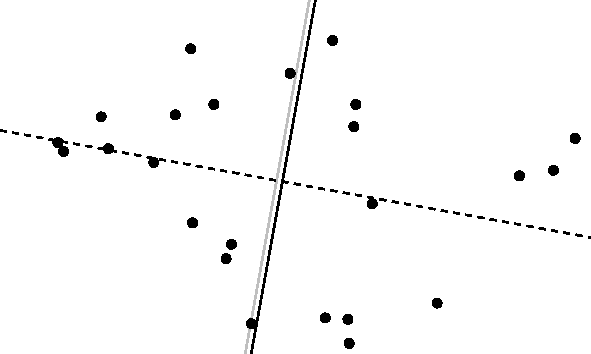
\includegraphics[width=0.85\linewidth]{RIB/RIB_diagram}
          \caption{
            Example of an inertial bisection.
            Vertices are shown as black points, the bisectors of the largest eigen-pair is shown by the black solid, and the bisector of the smallest eigen-pair is shown by the black dashed line.
            The ``shifted'' bisector used in the partitioning is shown in grey.
            While the communication between vertices is not drawn, it is clear that the length (proportional to cut size) of the smallest eigen-pair bisector is larger than that of the largest eigen-pair bisector.
            \label{fig:Spatial Decomposition:RIB Diagram}
          }
        \end{figure}
      }
      %%%%%%%%%%%%%%%%%%%%%%%%%%%%%%%%%%%%%%%%%%%%%%%%%%%%%%%%%%%%%%%%%%%%%%%%%%
      % Recursive Expansion-Based Methods
      %%%%%%%%%%%%%%%%%%%%%%%%%%%%%%%%%%%%%%%%%%%%%%%%%%%%%%%%%%%%%%%%%%%%%%%%%%
      \subsubsection{Recursive Expansion-Based Methods}{\label{sssec:Spatial Decomposition:Recursive Expansion-Based Methods}
        The \ac{REB} methods comprise the last class of partitioning methods examined in this work.
        These methods begin a bisection step by selecting a vertex as the starting point of a subdomain.
        This subdomain is then expanded until it is approximately half the size of the graph \cite{Farhat1988,Nasra1991,Elsner1997,Fitzgerald2017}.
        In this work, the method outlined by \citet{Fitzgerald2017} was slightly modified and generalized to weighted graphs.
        For the remainder of this work, the acronym \emph{\ac{REB}} will be used to denote this specific expansion-based method rather than the entire class of methods.

        This \ac{REB} method considers both the geometry and connectivity of the graph.
        The method begins by choosing a starting vertex for the subdomain and then expands based on a set of prioritized rules.
        At each expansion step, the next vertex is chosen so that it is geometrically close to the vertices within the subdomain and to minimize edges between the subdomain and the remaining graph.
        However, this method makes the assumptions that the mesh is structured, and that every mesh element is the same shape and size.
        For the application in MPACT, this is always true.

        This \ac{REB} method uses the concept of a \emph{\ac{SOI}} around a vertex.
        The \ac{SOI} includes directly neighboring vertices and vertices that neighbor more than one of the direct neighbors or that would if the direct neighbor were present in each structured position around the primary vertex.
        This is shown for 2-D rectangular structured mesh in \cref{fig:Spatial Decomposition:Sphere of Influence}.
        For implementation simplicity, the sphere of influence is calculated using distance rather than connectivity.

        The starting vertex in this \ac{REB} method is chosen using a set of prioritized rules:
        \begin{enumerate}
            \item{must be on graph boundary, i.e. at least one direct neighbor is not present,}
            \item{must have the lowest summed weight of edges, and}
            \item{must be located furthest from weighted centroid (given by \cref{eq:Spatial Decomposition:Mean Coordinates}).}
        \end{enumerate}
        Vertices within the expanding subdomain are considered internal vertices, and the remaining vertices are considered to be external vertices.
        During expansion, the next vertex is determined using a set of prioritized rules:
        \begin{enumerate}
            \item{must be neighboring at least one internal vertex,}
            \item{must have the highest summed weight of edges with internal vertices,}
            \item{must have the lowest summed weight of edges with external vertices,}
            \item{must have the largest number of internal SOI vertices,}
            \item{must have the largest number of external SOI vertices, and}
            \item{must have the smallest distance from reference vertex.}
        \end{enumerate}
        The reference vertex is in the expanding subdomain, which begins as the first vertex but changes during expansion; the reference vertex is the most recently added vertex with less external communication than the previously added vertex.
        An example of the expansion order is shown in \cref{fig:Spatial Decomposition:REB Expansion Order}.

        \begin{algorithm}
          \centering
          \caption{The chosen Recursive Expansion Bisection (REB) algorithm.}
          \label{alg:Recursive Expansion Bisection}
          \begin{algorithmic}[1]
            \Procedure{REB}{$G(V,E)$}
              \State{Compute weighted centroid of the graph}
              \State{Choose a starting vertex for the expanding domain: See rules in \cref{sssec:Recursive Expansion-Based Methods}}
              \State{Expand the domain from the starting vertex. Let $V_s$ be the list of vertices in order of the expansion: See rules in \cref{sssec:Recursive Expansion-Based Methods}}
              \State{Cut graph into $G_1(V_1,E_1), G_2(V_2,E_2)$: \Cref{alg:Graph Cutting}}
              \State{REB($G_1(V_1,E_1)$)}
              \State{REB($G_2(V_2,E_2)$)}
            \EndProcedure
          \end{algorithmic}
        \end{algorithm}

        \begin{figure}
          \centering
          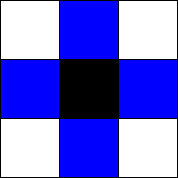
\includegraphics[width=0.45\linewidth]{REB/SoI_Rectangular}
          \caption{
              ``Sphere of influence'' example for 2D rectangular structured grid.
              The primary vertex is shown in black, direct neighbors are blue, and additional vertices in the sphere are white \cite{Fitzgerald2017}.
              \label{fig:Spatial Decomposition:Sphere of Influence}
          }
        \end{figure}

        \begin{figure}
          \centering
          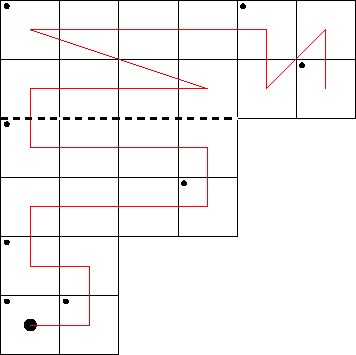
\includegraphics[width=0.65\linewidth]{REB/Expansion}
          \caption{
              An example of the REB method expansion on a small graph.
              The black lines show the square mesh cells.
              The expansion begins at the large black point in the center of a cell, and the red line from this shows the expansion's order.
              Each small black dot in the upper left of a cell indicates the reference vertices during expansion.
              The thick black dashed line shows the bisecting cut.
              \label{fig:Spatial Decomposition:REB Expansion Order}
          }
        \end{figure}

      }
    }
  }
  %%%%%%%%%%%%%%%%%%%%%%%%%%%%%%%%%%%%%%%%%%%%%%%%%%%%%%%%%%%%%%%%%%%%%%%%%%%%%%
  % Applications for MPACT
  %%%%%%%%%%%%%%%%%%%%%%%%%%%%%%%%%%%%%%%%%%%%%%%%%%%%%%%%%%%%%%%%%%%%%%%%%%%%%%
  \section{Applications for MPACT}{\label{sec:Spatial Decomposition:Applications for MPACT}
    As described in \cref{sec:Spatial Decomposition:Spatial Decomposition in MPACT}, MPACT's spatial decomposition is performed on the ray-tracing module mesh.
    However, there are a couple of restrictions on spatial subdomains in MPACT.
    Each spatial subdomain must be contiguous, and cannot wrap around other spatial subdomains.
    To account for these restrictions, adaptations are made to the graph partitioning process.

    Due to restrictions in MPACT, at each recursive step, each subdomain in a bisection is made contiguous.
    If a partitioning method results in a noncontiguous subdomain, then each noncontiguous group of modules will be moved into the other subdomain except for the largest group.
    This fix is done at the expense of load-balance, but is necessary for these methods to be robust in MPACT.
    To ensure that no subdomain wraps around another, a fix is applied after the graph partitioning process.
    If a subdomain wraps around another, then the concave subdomain will be given the modules it wraps around.

    A group of ray-tracing modules in MPACT can be abstracted into a graph.
    Each vertex will have weight corresponding to the number of cells contained in the module.
    Edges can be drawn between directly neighboring ray-tracing modules.
    This represents communication in MPACT's MOC solver.
    Transport source iterations converge slowly, so MPACT relies on the \ac{CMFD} \cite{Smith1983} acceleration method.
    \ac{CMFD} acceleration is performed by constructing a sparse linear system based on the finite differenced diffusion operator and then solving for the largest eigenpair of that linear system.
    In MPACT, solving the linear system is handled by a third-party library, PETSc \cite{Petsc}.

    For 2-D simulations, the application of graph partitioning methods is clear: abstract the 2-D mesh into a graph for partitioning.
    However, for 3-D, there are additional concerns.
    MPACT's primary 3-D transport method is the 2D-1D method, in which the \ac{MOC} is used in the radial directions, and a lower-order solver couples axial planes \cite{Collins2016}.
    For 2D-1D simulations, MPACT currently restricts spatial domains to be aligned in both the radial and axial directions; this is due to implementation, and is not a general requirement of the methods.

    To comply with MPACT's restrictions on 3D spatial domains, the current approach is to axially average module weights (numbers of cells), perform a 2-D graph partitioning on a single plane, and apply the resulting partitioning to all axial planes.
    This approach will restrict the number of spatial domains to be an integer multiple of the number of planes.
    This axially and radially aligned scheme is expected to work well in many cases since reactor cores do not typically vary significantly in the axial direction.
    However, for some designs, this may not be true, and planes near the top or bottom of the core have significantly fewer cells; in these cases, high load imbalance is to be expected.

    It is possible to change MPACT's implementation to lift these alignment restrictions.
    If spatial domains were aligned in only the radial direction, there may be some benefit to load-balance.
    In this scheme, each axial plane can be assigned an appropriate number of processes, and a separate 2-D decomposition can be performed for each plane.
    This also lifts restrictions on the number of domains; the number of domains must only be greater than or equal to the number of planes.

    If all alignment restrictions were lifted on MPACT's spatial domains, then a direct partitioning of the 3-D core can be performed by abstracting the entire core to a graph.
    This scheme provides the most freedom and would be expected to give the most balanced decompositions.
    In MPACT's 2D-1D solver, the amount of data communicated radially is significantly larger than that communicated axially, so it may be advantageous to assign the edges connecting the neighboring modules in the axial direction lower weights than those in radial directions.
    By doing so, the overall communication would be expected to be decreased.

    \begin{figure}
      \centering
      \begin{subfigure}[t]{0.3\textwidth}
        \centering
        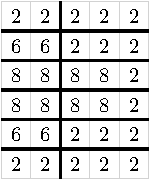
\includegraphics[width=0.9\textwidth]{alignmentComparison/pac_axial}
        \caption{}
      \end{subfigure}%
      ~
      \begin{subfigure}[t]{0.3\textwidth}
        \centering
        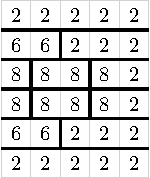
\includegraphics[width=0.9\textwidth]{alignmentComparison/pac_radial}
        \caption{}
      \end{subfigure}%
      ~
      \begin{subfigure}[t]{0.3\textwidth}
        \centering
        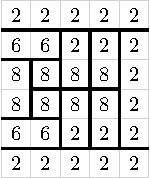
\includegraphics[width=0.9\textwidth]{alignmentComparison/pac_general}
        \caption{}
      \end{subfigure}
      \caption{
        Sample decompositions for (a) axially aligned, (b) radially aligned, and (c) generalized decomposition strategies.
        Rows represent axial planes.
        Numbers are the vertex weights.
        \label{fig:Spatial Decomposition:partitionAlignmentComparison}
      }
    \end{figure}

    \Cref{fig:partitionAlignmentComparison} shows a comparison of the three hypothetical decomposition schemes, for the purposes of illustration.
    Looking at the \ac{MMR}, as an indicator of load-balance, the strategies have clear differences.
    The \ac{MMR} for the axially aligned, radially aligned, and generalized strategies in this example are $4.00$, $2.67$, and $2.00$, respectively.
    However, it is important to note that the largest domain in each case has the same weight (16), so while the different schemes give different balances, the overall run-times are not expected to be different.
  }
  %%%%%%%%%%%%%%%%%%%%%%%%%%%%%%%%%%%%%%%%%%%%%%%%%%%%%%%%%%%%%%%%%%%%%%%%%%%%%%
  % Results
  %%%%%%%%%%%%%%%%%%%%%%%%%%%%%%%%%%%%%%%%%%%%%%%%%%%%%%%%%%%%%%%%%%%%%%%%%%%%%%
  \section{Results}{\label{sec:Spatial Decomposition:Results}
    %%%%%%%%%%%%%%%%%%%%%%%%%%%%%%%%%%%%%%%%%%%%%%%%%%%%%%%%%%%%%%%%%%%%%%%%%%%%
    % 2-D Results
    %%%%%%%%%%%%%%%%%%%%%%%%%%%%%%%%%%%%%%%%%%%%%%%%%%%%%%%%%%%%%%%%%%%%%%%%%%%%
    \subsection{2-D Results}{\label{ssec:Spatial Decomposition:2-D Results}
      \blindtext[8]
    }
    %%%%%%%%%%%%%%%%%%%%%%%%%%%%%%%%%%%%%%%%%%%%%%%%%%%%%%%%%%%%%%%%%%%%%%%%%%%%
    % 3-D Results
    %%%%%%%%%%%%%%%%%%%%%%%%%%%%%%%%%%%%%%%%%%%%%%%%%%%%%%%%%%%%%%%%%%%%%%%%%%%%
    \subsection{3-D Results}{\label{ssec:Spatial Decomposition:3-D Results}
      \blindtext[4]
    }
  }
  %%%%%%%%%%%%%%%%%%%%%%%%%%%%%%%%%%%%%%%%%%%%%%%%%%%%%%%%%%%%%%%%%%%%%%%%%%%%%%
  % Partition Refinement Methods
  %%%%%%%%%%%%%%%%%%%%%%%%%%%%%%%%%%%%%%%%%%%%%%%%%%%%%%%%%%%%%%%%%%%%%%%%%%%%%%
  \section{Partition Refinement}{\label{sec:Spatial Decomposition:Parition Refinement}
    \blindtext[8]
  }
  %%%%%%%%%%%%%%%%%%%%%%%%%%%%%%%%%%%%%%%%%%%%%%%%%%%%%%%%%%%%%%%%%%%%%%%%%%%%%%
  % Conclusions
  %%%%%%%%%%%%%%%%%%%%%%%%%%%%%%%%%%%%%%%%%%%%%%%%%%%%%%%%%%%%%%%%%%%%%%%%%%%%%%
  \section{Conclusions}{\label{sec:Spatial Decomposition:Conclusions}
    \blindtext[4]
  }
}